\section{The idea behind Column Generation}

% \todo{
% Structure: 1. Explain LP duality. 2. show that removing variables from primal = remove constraints from dual. 3. constraints is easier to check, with a partial solution
% of the primal we can map to the dual and check for constraints viaolation. if not violation optimal. maybe show concrete example before.
% }
% 
% 
% Strong duality \todo{ref} tell us that there exists another LP, called the dual, and that for any feasible solution $x$
% of the primal

We now describe how we used Column Generation (CG) \cite{desaulniers2006column} to overcome the model size problems faced when using the path model for
solving the traffic engineering problem with SR. CG is usually used to solve linear programs with a huge number of variables. The idea is to solve the problem for a subset
of the variables and then incrementally insert the missing variables, slowly growing the model. Each time that we add new variables, we solve the model again to check
for optimality. One could ask what
is the point of doing this since at some point we will have the whole set of variables, so why not just solve the full problem instead? However, we will carefully select the 
new variables that we introduce so that in general this framework will reach an optimal solution to the original \emph{problem without ever needing to consider all variables}.

To understand the impact of ignoring a variable and how we can prove optimality without considering all variables, we work out a small example. 
This will allow us to explain the main idea behind CG in a much more 
intuitive way by providing an example without overwhelming mathematical notations. Suppose that we have the following LP that we want to solve.

\begin{center}
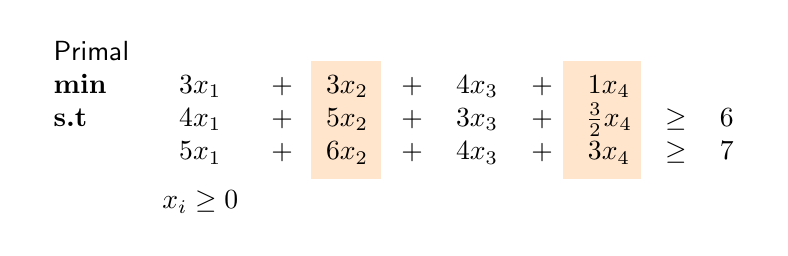
\begin{tikzpicture}
\def\x{0}
\def\y{0}
\fill[orange!20!white] (\x + 4 - 0.4, \y + 0 - 0.425) rectangle (\x + 4.9 - 0.4, \y + -1.5 - 0.425);
\fill[orange!20!white] (\x + 7.2 - 0.4, \y + 0 - 0.425) rectangle (\x + 8.1 - 0.3, \y + -1.5 - 0.425);
\node[anchor=north west] (primal) at (\x, \y) {
\begin{tabular}{lcccccccccc}
\textsf{Primal} & & & & & & & & & \\
$\displaystyle \mathbf{min}$ & $3 x_1$ & $+$ & $3 x_2$ & $+$ & $4 x_3$ & $+$ & $1 x_4$ & & \\
\textbf{s.t} & $4 x_1$ & $+$ & $5 x_2$ & $+$ & $3 x_3$ & $+$ & $\frac{3}{2} x_4$ & $\geq$ & $6$ \\
             & $5 x_1$ & $+$ & $6 x_2$ & $+$ & $4 x_3$ & $+$ & $3 x_4$ & $\geq$ & $7$ \\[0.2cm]
& $x_i \geq 0$ & & & & & & & &
\end{tabular}
};
\end{tikzpicture}
\end{center}

The dual of this problem can be obtained by following a systematic procedure. By doing so, we obtain the following linear program.
\begin{center}
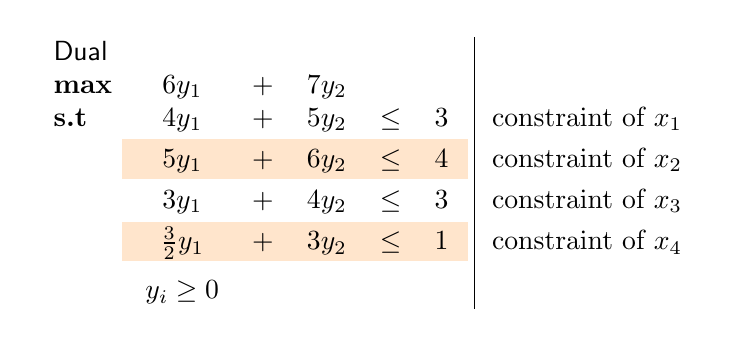
\begin{tikzpicture}
\def\x{0}
\def\y{0}
\fill[orange!20!white] (\x + 2 - 0.8, \y + -1 - 0.425) rectangle (\x + 5.6, \y + -1.5 - 0.425);
\fill[orange!20!white] (\x + 2 - 0.8, \y + -1.2 - 3 * 0.425) rectangle (\x + 5.6, \y + -1.7 - 3 * 0.425);
\node[anchor=north west] (dual) at (\x, \y) {
\begin{tabular}{lccccc | r}
\textsf{Dual} & & & & & \\
$\mathbf{max}$ & $6 y_1$ & $+$ & $7 y_2$ & &  \\
\textbf{s.t} & $4 y_1$ & $+$ & $5 y_2$ & $\leq$ & $3$ \quad & constraint of $x_1$ \\[0.1cm]
             & $5 y_1$ & $+$ & $6 y_2$ & $\leq$ & $4$ \quad  & constraint of $x_2$ \\[0.1cm]
             & $3 y_1$ & $+$ & $4 y_2$ & $\leq$ & $3$ \quad  & constraint of $x_3$ \\[0.1cm]
             & $\frac{3}{2} y_1$ & $+$ & $3 y_2$ & $\leq$ & $1$  \quad  & constraint of $x_4$ \\[0.2cm]
& $y_i \geq 0$ & & & &
\end{tabular}
};
\end{tikzpicture}
\end{center}

Each variable $x_i$ of the primal corresponds to a constraints of the dual. So, for instance, $x_2$ corresponds to constraint
$5 y_1 + 6 y_2 \geq 4$ and $x_4$ corresponds to the constraint $\frac{3}{2} y_1 + 3 y_2 \geq 1$ as highlighted in the models.

Because of this correspondence, when we ignore a variable on the primal, this translates in the dual to ignoring the corresponding constraint. 
For example, if we consider the restricted primal problem on variables $x_1$ and $x_3$ only (that we denote by $\textsf{Primal}(1, 3)$), 
and we take the dual, the dual will be the same as above but 
will only have the first and third constraints.

\begin{center}
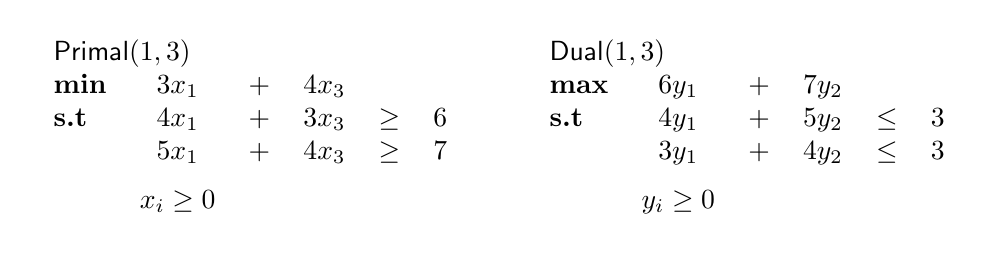
\begin{tikzpicture}
\def\x{0}
\def\y{0}
\node[anchor=north west] (primal) at (\x, \y) {
\begin{tabular}{lcccccccccc}
\multicolumn{11}{l}{$\textsf{Primal}(1, 3)$} \\
$\mathbf{min}$ & $3 x_1$  & $+$ & $4 x_3$ & & \\
\textbf{s.t} & $4 x_1$  & $+$ & $3 x_3$ & $\geq$ & $6$ \\
& $5 x_1$ & $+$ & $4 x_3$ & $\geq$ & $7$ \\[0.2cm]
& $x_i \geq 0$ & & & &
\end{tabular}
};

\def\x{6.3}
\def\y{0}
\node[anchor=north west] (dual) at (\x, \y) {
\begin{tabular}{lccccc}
\multicolumn{6}{l}{$\textsf{Dual}(1, 3)$} \\
$\mathbf{max}$ & $6 y_1$ & $+$ & $7 y_2$ & &  \\
\textbf{s.t} & $4 y_1$ & $+$ & $5 y_2$ & $\leq$ & $3$ \\
& $3 y_1$ & $+$ & $4 y_2$ & $\leq$ & $3$ \\[0.2cm]
& $y_i \geq 0$ & & & &
\end{tabular}
};
\end{tikzpicture}
\end{center}

Suppose that we solve the restricted primal we obtain the optimal solution $x^* = (1.5, 0)$. By duality, we also obtain 
an optimal solution $y^*$ of the restricted dual. In this case $y^* = (0.75, 0)$. From here, we want to be able to decide whether $x^*$ is actually optimal
for the original primal problem and, if not, what new variable $x_2$ or $x_4$ should we consider to improve the solution. By strong
duality, we know that $x^*$ is optimal for \textsf{Primal} if and only if $y^*$ is optimal for \textsf{Dual}. Since the only 
difference between \textsf{Dual} and $\textsf{Dual}(1, 3)$ is that we removed two constraints from \textsf{Dual}, $y^*$
contains values for \emph{all} variables of the dual. Therefore,
to check the optimality of $y^*$ for \textsf{Dual}, we can plug its values into the missing constraints to check whether $y^*$ satisfies them. 
If $y^*$ happens to satisfy all of them, then it must be optimal for the unrestricted dual and by consequence, $x^*$ is optimal for the
unrestricted original primal.
In this example, for the constraint corresponding to $x_2$ we have
\begin{align*}
5 y_1 + 6 y_2 = 5 \cdot 0.75 + 6 \cdot 0 = 3.75 > 3
\end{align*}
and for the constraint corresponding to $x_4$ we have
\begin{align*}
2 y_1 + 6 y_2 = 2 \cdot 0.75 + 6 \cdot 0 = 1.5 > 1. \\
\end{align*}
Both of them are violated so we cannot conclude that $y^*$ is optimal for \textsf{Dual}. So we chose one of $x_2, x_4$ to be added to the model.
For the sake of example, we choose $x_2$ obtaining (we highlighted in green the newly added column):

\begin{center}
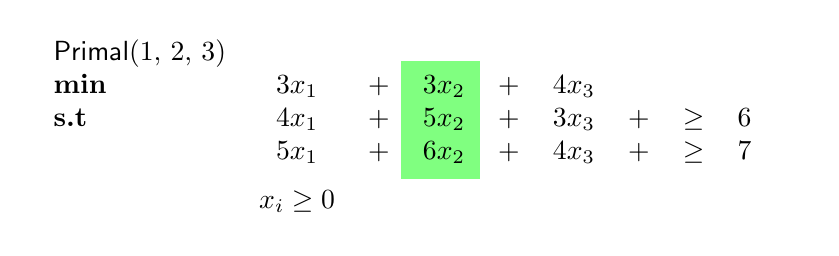
\begin{tikzpicture}
\def\x{0}
\def\y{0}
\fill[green!50!white] (\x + 4 + 1.15 - 0.4, \y + 0 - 0.425) rectangle (\x + 5 + 1.15 - 0.4, \y + -1.5 - 0.425);
\node[anchor=north west] (dual) at (\x, \y) {
\begin{tabular}{lcccccccccc}
\textsf{Primal}(1, 2, 3) & & & & & & &  \\
$\displaystyle \mathbf{min}$ & $3 x_1$ & $+$ & $3 x_2$ & $+$ & $4 x_3$ & & \\
\textbf{s.t} & $4 x_1$ & $+$ & $5 x_2$ & $+$ & $3 x_3$ & $+$ & $\geq$ & $6$ \\
             & $5 x_1$ & $+$ & $6 x_2$ & $+$ & $4 x_3$ & $+$ & $\geq$ & $7$ \\[0.2cm]
& $x_i \geq 0$ & & & & & & & &
\end{tabular}
};
\end{tikzpicture}
\end{center}

Solving this yields a primal solution $x^* = (0, 1.2, 0)$ and dual solution
$y^*(0.6, 0)$. As before, we check whether this solution is optimal for the 
original problem by checking whether it satisfies the remaining constraints.
In this case we only have one constraint left, the one corresponding to $x_4$.
By plugging into it the values of $y^*$ we get
\begin{align*}
\frac{3}{2} y_1 + 3 y_2 = \frac{3}{2} \cdot 0.6 + 3 \cdot 0 = 0.9 \leq 1. \\
\end{align*}
The constraint is satisfied so we conclude that $y^*$ is optimal for
\textsf{Dual} and by strong duality we conclude that $x^* = (0, 1.2, 0, 0)$
is optimal for \textsf{Primal} (note that we added a value of $0$ for 
all ignored variables).

With this process, we were able to solve \textsf{Primal} without ever having
to consider $x_4$. Of course this is just a small illustrative example so the gain is not
significant but, on larger models with a huge amount of variables, this can save huge amounts of computation
time. This finished our introductory example about column generation. 

We are now going to abstract from it and describe the general approach. Lets write the problem we are aiming to solve
in the following general form

\begin{center}
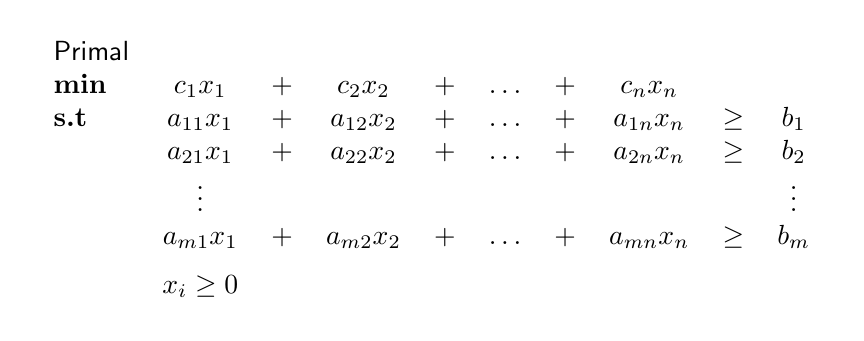
\begin{tikzpicture}
\def\x{0}
\def\y{0}
\node[anchor=north west] (primal) at (\x, \y) {
\begin{tabular}{lcccccccccc}
\textsf{Primal} & & & & & & & & & \\
$\displaystyle \mathbf{min}$ & $c_1 x_1$ & $+$ & $c_2 x_2$ & $+$ & $\ldots$ & $+$ & $c_n x_n$ & & \\
\textbf{s.t} & $a_{11} x_1$ & $+$ & $a_{12} x_2$ & $+$ & $\ldots$ & $+$ & $a_{1n} x_n$ & $\geq$ & $b_1$ \\
             & $a_{21} x_1$ & $+$ & $a_{22} x_2$ & $+$ & $\ldots$ & $+$ & $a_{2n} x_n$ & $\geq$ & $b_2$ \\
             & $\vdots$ & & & & & & & & $\vdots$ \\
             & $a_{m1} x_1$ & $+$ & $a_{m2} x_2$ & $+$ & $\ldots$ & $+$ & $a_{mn} x_n$ & $\geq$ & $b_m$ \\[0.2cm]
& $x_i \geq 0$ & & & & & & & &
\end{tabular}
};
\end{tikzpicture}
\end{center}

whose dual is easily shown to be

\begin{center}
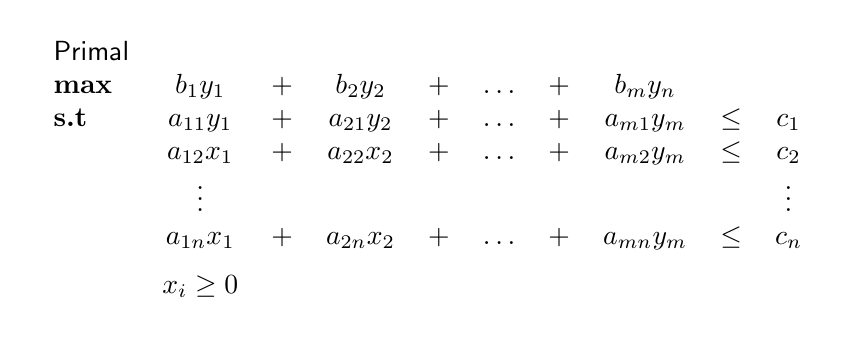
\begin{tikzpicture}
\def\x{0}
\def\y{0}
\node[anchor=north west] (primal) at (\x, \y) {
\begin{tabular}{lcccccccccc}
\textsf{Primal} & & & & & & & & & \\
$\displaystyle \mathbf{max}$ & $b_1 y_1$ & $+$ & $b_2 y_2$ & $+$ & $\ldots$ & $+$ & $b_m y_n$ & & \\
\textbf{s.t} & $a_{11} y_1$ & $+$ & $a_{21} y_2$ & $+$ & $\ldots$ & $+$ & $a_{m1} y_m$ & $\leq$ & $c_1$ \\
             & $a_{12} x_1$ & $+$ & $a_{22} x_2$ & $+$ & $\ldots$ & $+$ & $a_{m2} y_m$ & $\leq$ & $c_2$ \\
             & $\vdots$ & & & & & & & & $\vdots$ \\
             & $a_{1n} x_1$ & $+$ & $a_{2n} x_2$ & $+$ & $\ldots$ & $+$ & $a_{mn} y_m$ & $\leq$ & $c_n$ \\[0.2cm]
& $x_i \geq 0$ & & & & & & & &
\end{tabular}
};
\end{tikzpicture}
\end{center}

In general, we need a better way
for finding a new variable to introduce. In the previous example we did it by iterating over all remaining variables
and checking the corresponding constraint. Since CG is a framework that we want to use when we have a \emph{huge} amount of 
variables, this process is not realistic as it will involve checking the same amount of constraints. The idea to overcome this
is to express the problem of finding the variable as a another optimization problem which hopefully translates into something
that is solvable by an algorithm that is faster than a simple brute-force iterations on the missing variables.

The first step to achieve this is to express the condition for a new variable to be a candidate mathematically. Keeping the notation
used in the example, we see that each variable $x_i$ is associated to a column of coefficients $c_i, a_{1i}, a_{2i}, \ldots, a_{mi}$
where the first is the objective function coefficient and the others are the constraints coefficients in the primal.
The constraint associated to $x_i$ is the dual is given by
$$
a_{1i} + a_{2i} + \ldots + a_{mi} = \sum_{j = 1}^m a_{ji} y_i \leq c_i.
$$
Checking whether it is violated, or in other words, whether $x_i$ needs to be considered in the \textsf{Primal}, consists of 
checking whether
$$
\sum_{j = 1}^m a_{ji} y_i > c_i \Leftrightarrow \sum_{j = 1}^m a_{ji} y_i - c_i > 0.
$$

If we let $I$ be the set of indexes of the variables that we consider at a given point in the \textsf{Primal}, then the problem
of finding a new variable can be expressed as finding $i \in \{ 1, \ldots, n\} \setminus I$ such that
$$
\sum_{j = 1}^m a_{ji} y_i - c_i > 0.
$$
Therefore, if we compute the index $i^* \in \{ 1, \ldots, n\} \setminus I$ for which the value
$$
\sum_{j = 1}^m a_{ji^*} y_{i^*} - c_{i^*}
$$
is \emph{maximum} we know that there exists a new variable that we need to consider if and only if
$$
\sum_{j = 1}^m a_{ji^*} y_{i^*} - c_{i^*} > 0.
$$

Therefore, we can solve the problem of finding a new variable to add by solving the problem
$$
\max_{i \in \{ 1, \ldots, n\} \setminus I} \quad \sum_{j = 1}^m a_{ji} y_{i} - c_{i}.
$$
At first sight this problem might not seem any easier to solve than iterating over all $i \in \{ 1, \ldots, n\} \setminus I$
and computing the maximum but in practice this problem ofter has a nice structure and is usually solvable 
by a better, more efficient, algorithm than a simple brute force iteration. This problem is often referred to as the
\emph{pricing problem}.

Figure \ref{fig:col-gen-schema} provides a schematic vision of the column generation process.
CG generation is a very wide field and what we described here is just a very small glimpse into it \cite{desaulniers2006column}.
It is also important to note that what we did here only applies to \emph{continuous} linear programs and not to integer programming.
Therefore, we can only use this to compute solutions of LP that contain no integer variables. In order to obtain optimal
integral solution we need to add another layer to the algorithm and perform, for instance, a branch-and-price \cite{branchPrice}.
We did not explore this in this thesis but we believe that it would be interesting future work to see how fast we can
compute optimal solutions using this approach. 

In this thesis we instead use an heuristic algorithm to round the fractional solution getting an approximated solution rather
than an optimal one. %\todo{maybe we are going to explain branch-and-? also, if we find our notes}

\begin{figure}
\begin{center}
\begin{tikzpicture}
\node[draw, rounded corners, inner sep=0.25cm] (start) at (0, 0) {
  \begin{varwidth}{4cm}
    Select an initial set of variables $I$ such that \textsf{Primal}($I$)
    is feasible.
  \end{varwidth}
};

\node[draw, below= 1cm of start, rounded corners, inner sep=0.25cm] (lpsolve) {
  \begin{varwidth}{4cm}
    Solve \textsf{Primal}($I$) obtaining the primal and dual solutions $x^*, y^*$
  \end{varwidth}
};

\node[draw, below= 1cm of lpsolve, rounded corners, inner sep=0.25cm] (pricing) {
  \begin{varwidth}{4cm}
    Compute $i^* \in \{ 1, \ldots, n\} \setminus I$ such that $\sum_{j = 1}^m a_{ji} y_{i} - c_{i}$
    is maximum
  \end{varwidth}
};


\node[draw, right= 4cm of pricing, rounded corners, inner sep=0.25cm] (add) {
  \begin{varwidth}{4cm}
    Add $i^*$ to $I$
  \end{varwidth}
};

\node[draw, below= 2cm of pricing, rounded corners, inner sep=0.25cm] (quit) {
  \begin{varwidth}{4cm}
    $x^*$ with is the optimal solution of \textsf{Primal} (with value $0$ on
    variables outside of $I$)
  \end{varwidth}
};


\draw[line width=2] (start) edge[->] (lpsolve);

\draw[line width=2] (lpsolve) edge[->] (pricing);

\draw[line width=2] (pricing) edge[->, above] node {$\sum_{j = 1}^m a_{ji} y_{i} - c_{i} > 0$} (add);
\draw[line width=2] (add) -- ++(0, 2.65) edge[->] (lpsolve);

\draw[line width=2] (pricing) edge[->]  node[anchor=west] {$\sum_{j = 1}^m a_{ji} y_{i} - c_{i} \leq 0$} (quit);

\end{tikzpicture}
\end{center}
\caption{The CG framework used in this thesis.}
\label{fig:col-gen-schema}
\end{figure}

\section{CG for the path model}

We apply the process that we described above to the path model for the TE problem. As we mentioned before,
this model has a huge amount of variables since we have one variable per sr-path in $\Pk$ and $|\Pk| = O(|G|^k)$. Recall that 
the path model is obtained by replacing $\PB$ by $\Pk$ on the formulation of \bhatia.

\begin{center}
\begin{tabular}{crcllr}
\multicolumn{5}{l}{$\srtepath(G, \mathcal{D})$} \\[0.5cm] 
$\displaystyle \mathbf{min} \quad \lambda$ & & & & & \\[0.5cm]
$\textbf{s.t.}$ & $\displaystyle \sum_{\sr{p} \in \Pk} x_{d \sr{p}}$ & $=$ & $1$ & $\forall d \in \mathcal{D}$ \\[0.5cm] 
& $\displaystyle \sum_{\sr{p} \in \Pk} \sum_{d \in \mathcal{D}} \r(\sr{p}, e)  \cdot \vol(d) \cdot x_{d \sr{p}}$ & $\leq$ & $\lambda \cdot \bnd(e)$ & $\forall e \in E(G)$ \\[0.5cm]
& $x_{d\sr{p}} \in \{ 0, 1 \}$ & & & $\forall \sr{p} \in \Pk, \ \forall d \in \mathcal{D}$
\end{tabular}
\end{center}

Our experiments showed that working directly on the path model caused the column generation process described in Figure \ref{fig:col-gen-schema}
to require adding a lot of columns before proving optimality. It would get stuck with the same optimal value for the restricted problem
for huge number of iterations. For this reason we decided to formulate the problem with the same constraints but with the objective of routing
a maximum amount of demands for a given factor $\lambda$.

Since $x_{d \sr{p}}$ says whether demand $d$ is routed over sr-path $\sr{p}$, the total amount of traffic that is routed by a solution $x_{d\sr{p}}$ 
if given 
$$
\sum_{\sr{p} \in \Pk} \sum_{d \in \mathcal{D}} \vol(d) \cdot x_{d\sr{p}}.
$$

Routing a maximum demand volume thus amounts at maximizing this value. Putting it together with the constraints from the path model \srtepath~we obtain the 
following model.

\begin{center}
\begin{tabular}{crcll}
\multicolumn{5}{l}{$\displaystyle \srtepathdem(G, \mathcal{D}, \mathcal{P}, \lambda)$} \\[0.5cm] 
$\displaystyle \mathbf{max}$ & $\displaystyle \sum_{\sr{p} \in \Pk} \sum_{d \in \mathcal{D}} \vol(d) \cdot x_{dp}$ & & & \\[0.5cm]
$\textbf{s.t.}$ & $\displaystyle \sum_{\sr{p} \in \Pk} x_{d \sr{p}}$ & $\leq$ & $1$ & $\forall d \in \mathcal{D}$ \\[0.5cm] 
& $\displaystyle \sum_{\sr{p} \in \Pk} \sum_{d \in \mathcal{D}} \r(\sr{p}, e)  \cdot \vol(d) \cdot x_{d \sr{p}}$ & $\leq$ & $\lambda \cdot \bnd(e)$ & $\forall e \in E(G)$ \\[0.5cm] 
& $x_{d \sr{p}} \in \{0, 1\}$ & $\geq$ & $0$ & $\forall \sr{p} \in \Pk, \ \forall d \in \mathcal{D}$
\end{tabular}
\end{center}



In this formulation, $\lambda$ is a parameter that is given as input. We still want to minimize it so that we end up with a solution of Problem \ref{prob:srte}. However, we do not do this directly with linear programming, we instead perform a binary search on $\lambda$ to find the minimum lambda that is able to route \emph{all} demands.
The other difference relative to the original path model is that on the first set of constraints we now have an inequality rather than an equality. Both are equivalent.
This is the the case because, since the objective now is to route the maximum amount of demands, we always end up with a solution that selects one path per demand. The only reason for using
the inequality is that it simplifies a bit the process of finding the dual.

We apply the process described in our CG introduction to this problem. Since CG needs a LP and \srtepathdem~is a MIP, we first relax integrality constraints  
by replacing $x_{d \sr{p}} \in \{ 0, 1 \}$ by $x_{d \sr{p}} \geq 0$. Note that, again, the most natural would have been to say $x_{d \sr{p}} \in [0, 1]$ but saying $x_{d \sr{p}} \geq 0$ is equivalent
for this problem because of the first set of constraints. The reason for this choice is again that is makes the process of computing the dual simpler because it leaves the 
formulation in a standard form. We also need to add the current set of variables as a parameter. Since in our case variables correspond to sr-paths, we pass
as an argument a set of sr-paths $\mathcal{P}$ corresponding to the set of variables to which we restrict the problem. The CG process then slowly grow this
set until we reach an optimal solution. The linear programming relaxation we obtain is the following.

\begin{center}
\begin{tabular}{crcll}
\multicolumn{5}{l}{$\displaystyle \srtepathlp(G, \mathcal{D}, \mathcal{P}, \lambda)$} \\[0.5cm] 
$\displaystyle \mathbf{max}$ & $\displaystyle \sum_{\sr{p} \in \Pk} \sum_{d \in \mathcal{D}} \vol(d) \cdot x_{dp}$ & & & \\[0.5cm]
$\textbf{s.t.}$ & $\displaystyle \sum_{\sr{p} \in \Pk} x_{d \sr{p}}$ & $\leq$ & $1$ & $\forall d \in \mathcal{D}$ \\[0.5cm] 
& $\displaystyle \sum_{\sr{p} \in \Pk} \sum_{d \in \mathcal{D}} \r(\sr{p}, e)  \cdot \vol(d) \cdot x_{d \sr{p}}$ & $\leq$ & $\lambda \cdot \bnd(e)$ & $\forall e \in E(G)$ \\[0.5cm] 
& $x_{d\sr{p}}$ & $\geq$ & $0$ & $\forall \sr{p} \in \Pk, \ \forall d \in \mathcal{D}$
\end{tabular}
\end{center}

Since $\srtepathlp$ is already in standard form it is very easy to obtain its dual. In general, computing the dual
of a linear program can be achieved by following a systematic procedure. We omit the details here as this is quite a common process.
Doing so we obtain the following formulation for the dual.

\begin{center}
\begin{tabular}{crcll}
\multicolumn{5}{l}{$\displaystyle \srtepathlpdual(G, \mathcal{D}, \mathcal{P}, \lambda)$} \\[0.5cm] 
$\displaystyle \mathbf{min}$ & $\displaystyle \lambda \cdot \sum_{e \in E(G)} \bnd(e) \cdot y_e + \sum_{d \in \mathcal{D}} z_d$ & & & \\[0.5cm]
$\textbf{s.t.}$ & $z_d + \sum_{e \in E(G)} \r(\sr{p}, e) \cdot \vol(d) \cdot y_e$ & $\geq$ & $\vol(d)$ & $\forall \sr{p} \in \Pk$ \\[0.5cm] 
& $y_e, z_d$ & $\geq$ & $0$ & $\forall \sr{p} \in \Pk, \ \forall d \in \mathcal{D}$
\end{tabular}
\end{center}

The next step is to describe the pricing problem. By what we said above, this  corresponds to finding a sr-path $\sr{p} \in \Pk$ and a demand $d \in \mathcal{D}$
that violate the dual constraints, that is, such  that
\begin{align*}
z_d + \sum_{e \in E(G)} \r(\sr{p}, e) \cdot \vol(d) \cdot y_e < \vol(d) & \Leftrightarrow \\
\sum_{e \in E(G)} \r(\sr{p}, e) \cdot \vol(d) \cdot y_e < \vol(d) - z_d & \Leftrightarrow \\
\sum_{e \in E(G)} \r(\sr{p}, e) \cdot y_e < \frac{\vol(d) - z_d}{\vol(d)} & \\
\end{align*}
If such $\sr{p}$ and $d$ exist then we will add $\sr{p}$ to the $\mathcal{P}$. If not, then, by what we said above, we know that the optimal solution for the restricted sr-path set $\mathcal{P}$
is also optimal for the complete sr-path set $\Pk$.

\begin{problem}{SRTE pricing}
\label{prob:srte-pricing}
\textbf{Input:} A network $G$, a demand set $\mathcal{D}$, $k \geq \mathbb{N}$ and values $y_e \geq 0$ for each $e \in E(G)$.

\textbf{Output:} A sr-path $\sr{p} \in \Pk$ and a demand $d \in \mathcal{D}$ such that
$$
\sum_{e \in E(G)} \r(\sr{p}, e) \cdot y_e < \frac{\vol(d) - z_d}{\vol(d)}
$$
or report that no such path exists.
\end{problem}

\begin{theorem}
Problem \ref{prob:srte-pricing} can be solved in polynomial time. 
\end{theorem}

\begin{proof}
Let $d \in \mathcal{D}$.
Consider the sr-metric $c$ defined for all $u, v \in V(G)$ and $e \in E(G)$ as
$$
c(u, v) = \sum_{e \in E(G)} \r(u, v, e) \cdot y_e
$$
and
$$
c(e) = y_e.
$$
Let know that we can compute a sr-path $\sr{p} = \langle x_1, \ldots, x_l \rangle \in \Pk$ that minimizes
$$
c(\sr{p}) = \sum_{i = 2}^l c(x^2_{i - 1}, x^1_i) + \sum_{i : x_i \in E(G)} c(x_i)
$$
in polynomial time using Algorithm \ref{algo:min_weight_sr_path} from Chapter \ref{chapter:sr-optimal}. We have that
\begin{align*}
c(\sr{p}) & = \sum_{i = 2}^l c(x^2_{i - 1}, x^1_i) + \sum_{i : x_i \in E(G)} c(x_i) \\
& = \sum_{i = 2}^l  \sum_{e \in E(G)} \r(x^2_{i - 1}, x^1_i, e) \cdot y_e + \sum_{i : x_i \in E(G)} y_{x_i} \\
& = \sum_{e \in E(G)} \sum_{i = 2}^l \r(x^2_{i - 1}, x^1_i, e) \cdot y_e + \sum_{e \in E(G)} \sum_{i : x_i = e} y_{e} \\
& = \sum_{e \in E(G)} \left( \sum_{i = 2}^l \r(x^2_{i - 1}, x^1_i, e) \cdot y_e + \sum_{i : x_i = e} y_{e} \right) \\
& = \sum_{e \in E(G)} \left( \sum_{i = 2}^l \r(x^2_{i - 1}, x^1_i, e) + \sum_{i : x_i = e} 1 \right) \cdot y_e \\
& = \sum_{e \in E(G)} \r(\sr{p}, e)\cdot y_e.
\end{align*}
Since $\sr{p}$ has minimum cost, Problem \ref{prob:srte-pricing} has a solution if and only if
$$
c(\sr{p}) =  \sum_{e \in E(G)} \r(\sr{p}, e)\cdot y_e < \frac{\vol(d) - z_d}{\vol(d)}
$$
in which case $\sr{p}$ is a solution. Since Algorithm \ref{algo:min_weight_sr_path} runs in polynomial time, this means that
we can decide in polynomial time whether for a given demand $d \in \mathcal{D}$ there exists a sr-path $\sr{p}$ that violates the dual constraints.
Thus by iterating over all demands we get a polynomial time algorithm overall.
\end{proof}

With this theorem we have an example of a problem where finding a new variable to add can be done in a much more efficient way
than iterating over all remaining variables. Using the schema in Figure \ref{fig:col-gen-schema} we can then compute optimal
solutions to the LP relaxation \srtepathlp~of \srtepathdem.

The solution obtained with this process is optimal for Problem \ref{prob:srte-mul} and provides a lower bound form Problem \ref{prob:srte}.
In itself this is already a good result since those bounds are important for evaluating the quality of greedy solution. Until now, the
best lower bounds were computed using the MCF. The bounds obtained with the MCF are of lower quality since they do not take into account
segment routing as show at the end of this chapter.

\section{Minimizing the worst link utilization $\lambda$}

We saw in the previous section how to use CG to compute the maximum demand volume that we can route for a given 
capacity factor $\lambda$. In this section we explain how to use this as a sub-routine to compute the
minimum $\lambda$ for which we can route \emph{all} demands.

Let $\mathcal{V} = \sum_{d \in \mathcal{D}} \vol(d)$ be the total volume of demands in $\mathcal{D}$. To find the minimum
capacity factor perform a binary search on $\lambda \in [0, \lambda_M]$ where $\lambda_M$ is a big enough capacity factor
that ensure that all demands can be routed. For each $\lambda$ we solve $\srtepathdem(G, \mathcal{D}, P, \lambda)$. If the
solution is $\mathcal{V}$ then we continue the search with $\lambda$ as the new upper bound. Otherwise we set $\lambda$
as the new lower bound and continue. Each time we solve $\srtepathdem(G, \mathcal{D}, P, \lambda)$ we do not start from scratch. 
We continue the CG process with the set of paths $P$ from the previous iterations.

\subsubsection*{Initial sr-path set}

We need to select an initial feasible sr-path set $\mathcal{P}$. In this case, feasibility
is not an issue as we can select the capacity factor $\lambda_M$ so that it is large enough to make any solution with at least one sr-path per demand
feasible. To compute the initial path set, we use Algorithm \ref{algo:max_cap_sr_path} to compute the maximum capacity sr-path for each demand.

% For this reason we choose to use to start the algorithm with $\mathcal{P} = \left\{ \langle s, t \rangle \mid (s, t, \nu) \in \mathcal{D} \right\}$.
% Using an heuristic algorithm for selecting a better path set might improve the runtime of the algorithm. We did not explore this further in this thesis
% but we encourage people to do so if they want to implement this approach on real network. \todo{actually we did try the maximum capacity paths, should we talk about that?
% maybe in the min lat path chapter we can add some more stuff explaining how we can compute this}

\subsubsection*{Generating new paths}

We explained above that we can solve the pricing by iterating over all demands $d \in \mathcal{D}$ and computing a minimum cost sr-path for
specific weights that depend on the values $y, z$ of the dual solution. There might be several sr-path demand pairs $\sr{p}, d$ that violate
 the dual constraints and each such path corresponds to a new candidate variable that might improve the current solution if added. However,
if there are a lot of demands, computing the minimum cost sr-path for each and every one of them may be time consuming, even being a polynomial time procedure. Also, adding a lot of new paths
makes solving the relaxed problem slower since it will contain more variables. On the other hand, having more paths will maybe make the CG converge faster 
towards the optimal solution. Hence, we face a trade-off between adding more paths and making each iteration slower or adding fewer paths and having more iterations overall.

To have more control over this, we add a parameter to our algorithm $maxp$ that limits the number of sr-paths than can be generated in a single iteration.
At each CG iteration we loop over all the demands and for each of them check if it has a sr-path to be added. After $maxp$ demands yield a new sr-path we stop this iteration
and solve the new linear program obtained by adding these paths. The order in which we iterate over the demands should be such that we start with demands that have a higher
chance of yielding a sr-path that violates the dual constraints, that is, a sr-path $\sr{p}$ such that

$$
\sum_{e \in E(G)} \r(\sr{p}, e) \cdot y_e < \frac{\vol(d) - z_d}{\vol(d)}.
$$

Hence, we sort the demands by decreasing value of $\frac{\vol(d) - z_d}{\vol(d)}$ since the higher this value is, the more likely we are of finding a
sr-path whose weight lower cost. This is important since it helps avoiding useless time consuming invocations of the minimum cost sr-path algorithm.

\subsubsection*{Rounding heuristic}

As we explained above, at the end of the column generation process, we have an optimal solution for the relaxed master problem $\srtepathlp$ where variables can have fractional
values. In practice, this means that each demand might be split over several paths, in other words, we have an optimal segment routing solution for Problem \ref{prob:srte-mul}.
If we seek a solution from Problem \ref{prob:srte} we need to ensure that each demand is assigned to exactly one path. If sub-optimal solutions are acceptable, then an efficient
way to achieve this is to use some kind of heuristic to assign a path to each demand amongst the paths obtained in the end. We propose to do this by re-solving 
$\srtepath$ with integrality constraints using a MIP solver. As we discuss later, our experiments showed that in this way we obtain near optimal solutions to Problem \ref{prob:srte}.
This is an heuristic since, with integer variables, there is no guarantee that the restricted optimal solution is the optimal for the unrestricted problem.

By putting all these ideas together we can provide the following formal description of our column generation algorithm for the traffic engineering problem.
Algorithm \ref{algo:iterate} performs one iteration of the column generation algorithm. It starts on line \ref{line:mastersolve} by computing the optimal solution of the linear program
$\srtepathlp$ for the current sr-path set obtaining a primal solution $x$, the corresponding dual solution $y, z$ and the maximum value $vol$ that we can be routed on the current path set for the current capacity factor $\lambda$. Afterwards, from line \ref{line:coststart} to line \ref{line:costend} it computes the sr-metric used for the minimum cost sr-path computation. Then it iterates over all
demands and tries to find new paths to add. All those paths are put together and returned.

Algorithm \ref{algo:colgen} performs column generation iterations by calling Algorithm \ref{algo:iterate} until no new paths are found thus computing an optimal solution of 
$\srtepathlp(\mathcal{P}, \mathcal{D}, \lambda)$ for a given capacity factor $\lambda$ over the full sr-path set $\Pk$. Finally, Algorithm \ref{algo:SRGen} uses the column generation as a sub-routine 
on a binary search to find the smallest value of $\lambda$ such that the optimal solution of $\srtepathlp(\mathcal{P}, \mathcal{D}, \lambda)$ is equal to $\mathcal{V}$. In other words, it uses a binary
search combined with the column generation to find the smallest capacity factor that allows one to route the whole volume of demands.

\begin{algorithm}[t]
\small
\caption{$\textsf{iterate-CG}\left( G, \mathcal{P}, \mathcal{D}, \lambda, \textit{maxp} \right)$}
\begin{algorithmic}[1]
%\algrule
\STATE $x, (y, z)_x, \textit{vol} \gets \textsf{LP-solve}(\srtepathlp(\mathcal{P}, \mathcal{D}, \lambda))$ \label{line:mastersolve}
\FOR{$x, y \in V$} \label{line:coststart}
  \STATE $c(x, y) \gets \sum_{e \in E(\langle x, y \rangle)} \r(x, y, e) \cdot y_e$           
\ENDFOR
\FOR{$e \in E$}
  \STATE $c(e) \gets y_e$
\ENDFOR \label{line:costend}
\STATE $P' \gets \emptyset$
\FOR{$d \in \mathcal{D}$ \textbf{in decreasing order of $(\vol(d) - z_d) \slash \vol(d)$}}
  \STATE $p \gets \textsf{mincost-srpath}(s(d), t(d), c)$
  \IF{$c(p) < (v(d) - \delta_d) \slash v$}
    \STATE $P' \gets P' \cup \{ p \}$
  \ENDIF
  \IF{$|P'| \geq \textit{maxp}$}
    \STATE \textbf{break}
  \ENDIF
\ENDFOR
\RETURN $P'$
\end{algorithmic}
\label{algo:iterate}
\end{algorithm}

\begin{algorithm}[t]
\small
\caption{$\textsf{binsearch-CG}\left( \mathcal{D}, \lambda_M, k, \epsilon, \textit{maxp} \right)$}
\begin{algorithmic}[1]
%\algrule
\STATE $\mathcal{P} \gets \{ \textsf{maxCapSrPath}(g, \tau, s, t, k) \mid (s, t, d) \in \mathcal{D} \}$ \label{line:init}
\STATE $\mathcal{V} \gets \sum_{d \in \mathcal{D}} \vol(d)$
\STATE $lb \gets 0$
\STATE $ub \gets \lambda_M$
\WHILE{$|lb - ub| > \epsilon$}
  \STATE $\lambda \gets (lb + ub) \slash 2$
  \STATE $x, (y, z)_x, \textit{vol} \gets \textsf{column-generation}(\mathcal{P}, \mathcal{D}, \lambda, \textit{maxp})$
  \IF{$\textit{vol} = \mathcal{V}$}
    \STATE $lb \gets \lambda$
  \ELSE
    \STATE $ub \gets \lambda$
  \ENDIF
\ENDWHILE
\RETURN $\textsf{ILP-solve}(\srtepathdem(\mathcal{P}, \mathcal{D}))$ 
\end{algorithmic}
\label{algo:SRGen}
\end{algorithm}

\begin{algorithm}[t]
\small
\caption{$\textsf{column-generation}\left( \mathcal{P}, \mathcal{D}, \lambda, \textit{maxp} \right)$}
\begin{algorithmic}[1]
%\algrule
\WHILE{$P' \gets \textsf{iterate}(\mathcal{P}, \mathcal{D}, \lambda, \textit{maxp}) \neq \emptyset$}
  \STATE $\mathcal{P} \gets \mathcal{P} \cup P'$
\ENDWHILE
%\STATE $\primalx = \textsf{ILP-solve}(\primal(\P, \D, \lambda))$
\RETURN $\textsf{LP-solve}(\srtepathdem(G, \mathcal{D}, \mathcal{P}, \lambda))$
\end{algorithmic}
\label{algo:colgen}
\end{algorithm}
